% =============================================================================
% Capítulo 2 — Ocultações Estelares e Processamento de Dados Astronômicos
% =============================================================================
% Este capítulo fornece o arcabouço fenomenológico e observacional das ocultações
% estelares e das curvas de luz, em harmonia com a Introdução (contexto científico),
% o Cap. 3 (modelos de ML) e o Cap. 4 (metodologia e pipeline).
%\section{Objetivos do capítulo}
%\label{sec:objetivos_cap2}
Neste capítulo será discutida a fenomenologia das ocultações estelares, o papel da curva de luz na caracterização física dos corpos ocultantes e será descrito, em linhas gerais, como as observações são obtidas e armazenadas, de modo a situar a origem dos dados utilizados na \textit{pipeline} de detecção (detalhada no Capítulo 4). Além disso, serão definidas as principais características das curvas de luz - morfologia, detecção positiva versus negativa e fatores que afetam a forma do sinal - sem repetir a engenharia de características nem os modelos de ML, tratados nos capítulos seguintes.

% ---------------------------
\section{O que são Ocultações Estelares?}
\label{sec:fenomenologia}

Uma \textbf{ocultação estelar} ocorre quando um objeto celeste (planeta, satélite natural, asteroide ou objeto transnetuniano) passa na frente de uma estrela distante, bloqueando temporariamente parte ou toda a sua luz. Esse evento se manifesta como uma queda característica no fluxo luminoso registrado por um observador na Terra. Como a estrela ocultada está a distâncias muito maiores que a do corpo do Sistema Solar à Terra (a estrela em anos-luz, o corpo em horas-luz), os raios luminosos que chegam ao corpo são essencialmente paralelos: a sombra projetada na superfície terrestre preserva fielmente o limbo do corpo, com escala unitária. Essa projeção, combinada à alta resolução temporal das observações, permite determinar tamanho, forma projetada no plano do céu e, em casos favoráveis, atmosfera, anéis ou satélites do corpo ocultante, com precisão comparável à de sondas espaciais \citep{Sicardy2011, Knieling2024}.

\begin{figure}[htbp]
    \centering
    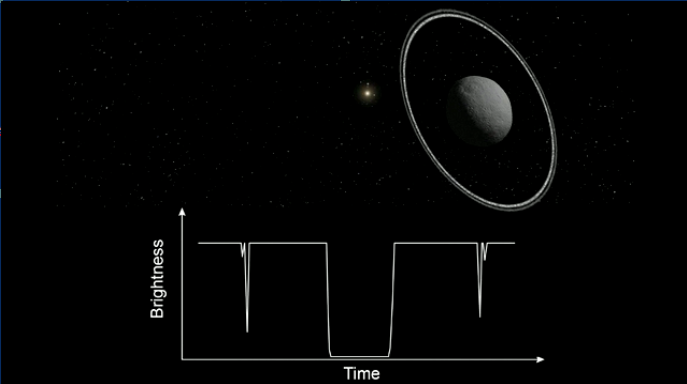
\includegraphics[scale=0.7]{pngs/curva.png}
    \caption{Representação artística de uma ocultação estelar pelo Centauro (10199)~Chariklo e seu sistema de anéis. A curva de luz esquemática (abaixo) mostra as quedas de fluxo correspondentes à passagem dos anéis e do corpo principal diante da estrela. Crédito: Lucie Maquet, 2014.}
    \label{fig:ilustracao_ocultacao}
\end{figure}

A sombra do corpo ocultante projeta-se na superfície terrestre. A precisão quilométrica decorre da combinação dessa projeção com a alta resolução temporal das observações. Cada observador, em sua posição geográfica, registra um intervalo de tempo durante o qual a estrela é ocultada - uma \textbf{corda} no plano do céu. A duração e o instante central da corda dependem da posição do observador em relação ao trajeto da sombra. Vários observadores em locais diferentes produzem várias cordas; a combinação dessas cordas permite reconstruir a forma e o tamanho do corpo no plano do céu com alta precisão \citep{SORA2022}. A previsão de ocultações depende criticamente da precisão das posições estelares e das efemérides do corpo; a melhoria contínua desses ingredientes tem ampliado o número de eventos previstos e observados, inserindo a técnica na era do \textit{big data} em astronomia \citep{SORA2022, Knieling2024}. Graças à precisão astrométrica do catálogo Gaia, o gargalo atual para a previsão de ocultações está na qualidade das efemérides dos pequenos corpos do Sistema Solar.

\begin{figure}[htbp]
    \centering
    \begin{minipage}[b]{0.48\textwidth}
        \centering
        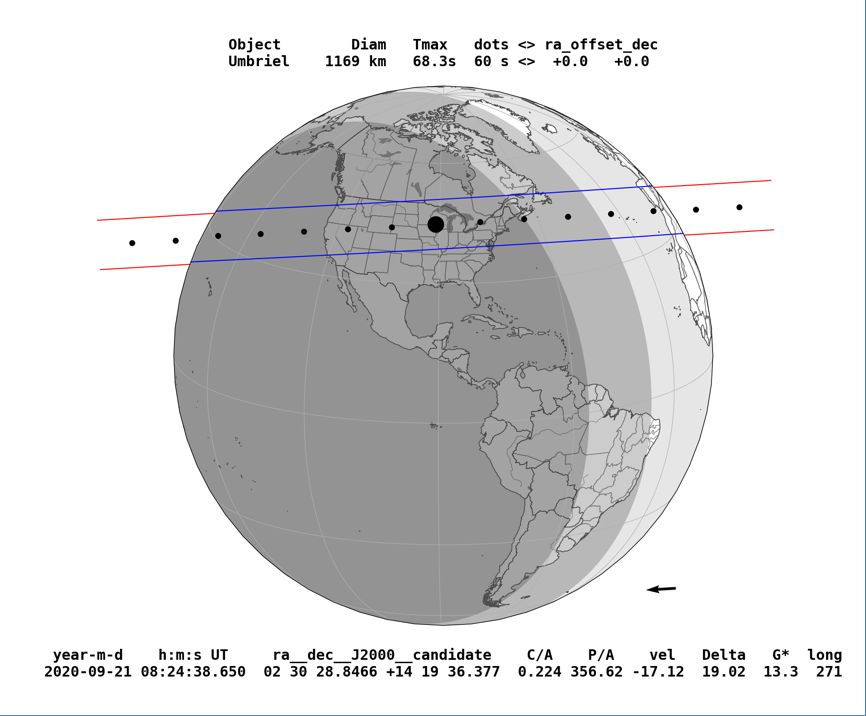
\includegraphics[width=\textwidth]{pngs/OccUmbriel_mapa.png}
        \centerline{\small (a)}
    \end{minipage}
    \hfill
    \begin{minipage}[b]{0.48\textwidth}
        \centering
        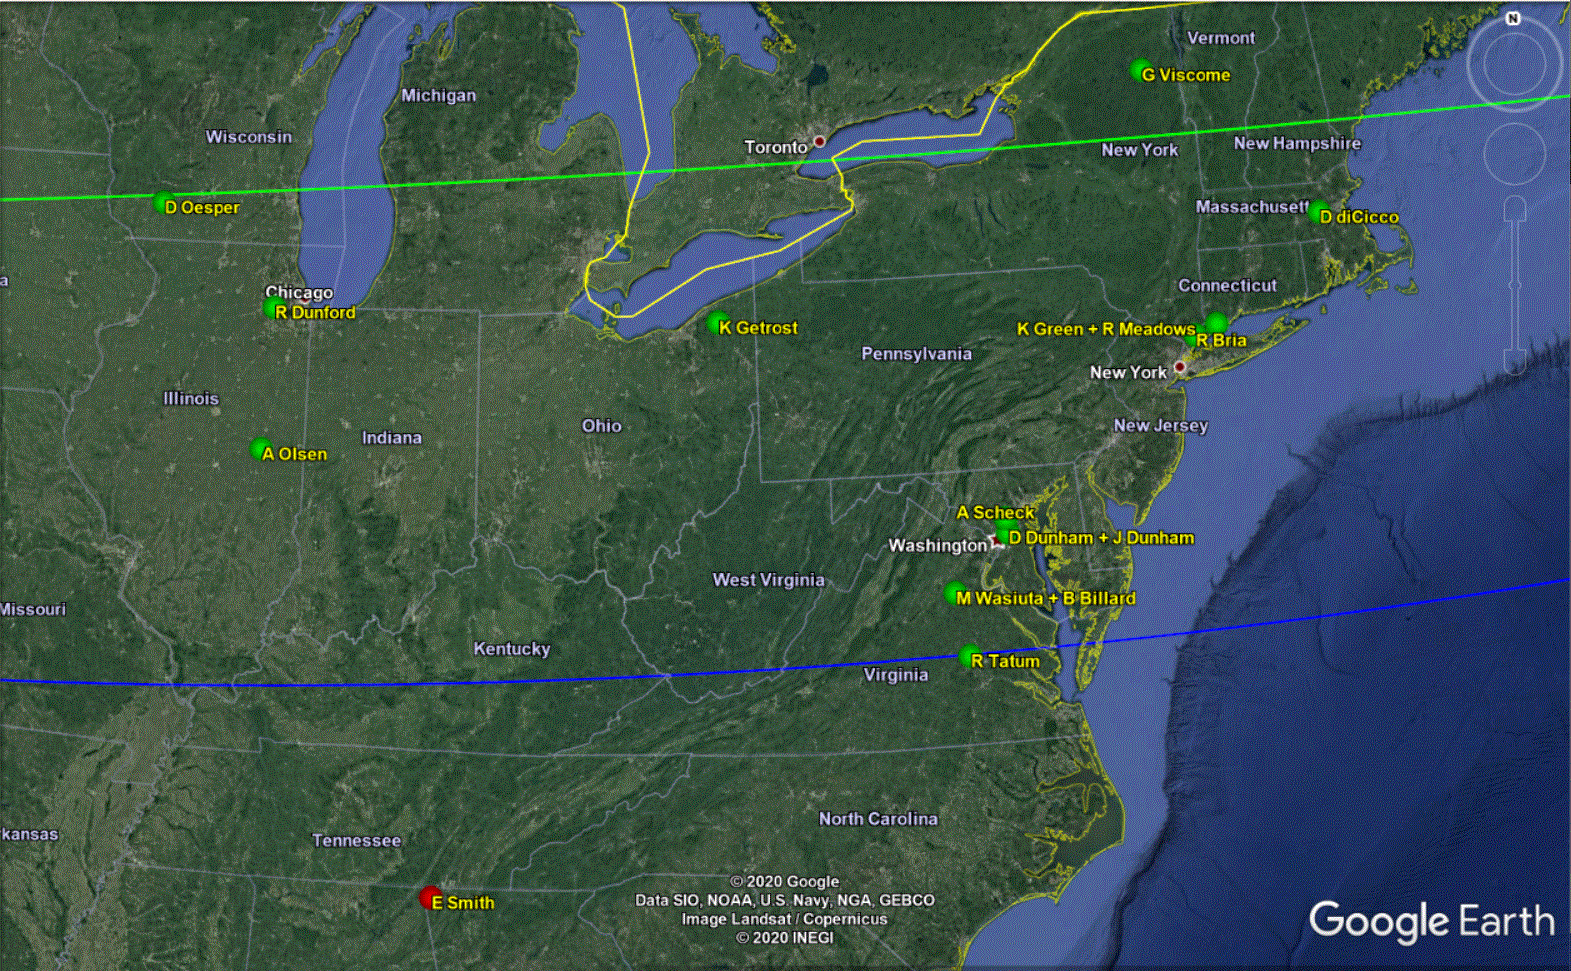
\includegraphics[width=\textwidth]{pngs/OccUmbriel_mapa2.png}
        \centerline{\small (b)}
    \end{minipage}

    \vspace{0.4cm}

    \begin{minipage}[b]{0.48\textwidth}
        \centering
        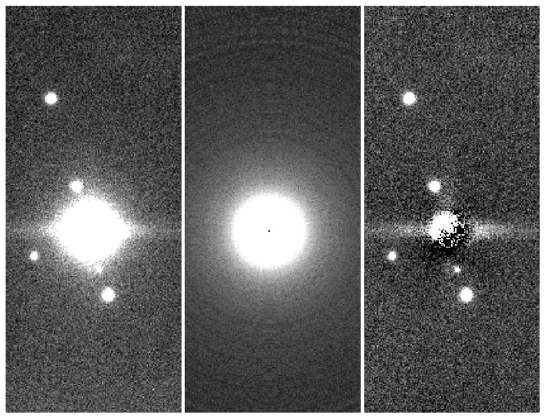
\includegraphics[width=\textwidth]{pngs/OccUmbriel_outputExemplo.png}
        \centerline{\small (c)}
    \end{minipage}
    \hfill
    \begin{minipage}[b]{0.48\textwidth}
        \centering
        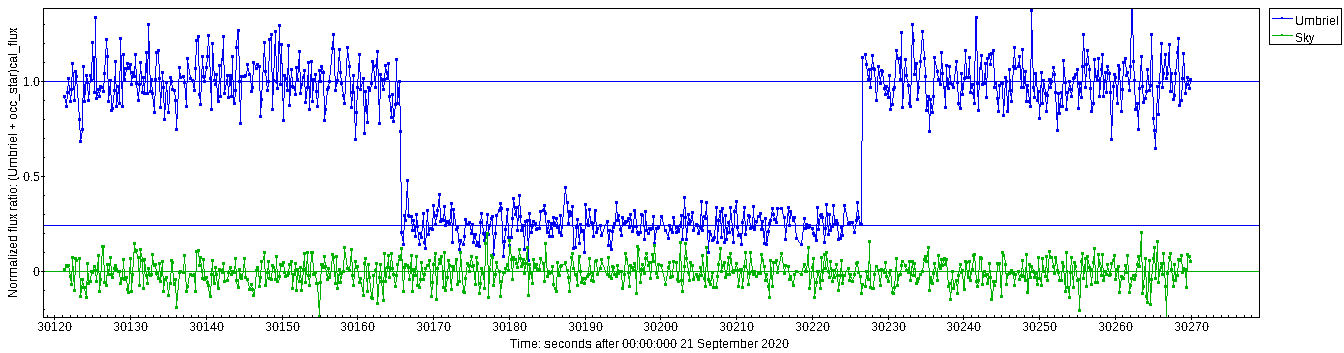
\includegraphics[width=\textwidth]{pngs/OccUmbriel_outputExemplo2.png}
        \centerline{\small (d)}
    \end{minipage}
    \caption{Exemplo completo do fluxo observacional: ocultação estelar por Umbriel (satélite de Urano), observada em 21 de setembro de 2020 \citep{Umbriel2020}. (a)~Mapa de previsão da sombra sobre a superfície terrestre. (b)~Detalhe do posicionamento dos observadores na costa leste dos EUA (Google Earth). (c)~Exemplo de quadros CCD obtidos por uma das estações: são imagens como estas que alimentam os pacotes de fotometria (e.g.\ PRAIA) para a construção das curvas de luz. Neste caso, o brilho intenso de Urano exigiu a aplicação de coronagrafia digital para viabilizar a fotometria precisa de Umbriel. (d)~Curva de luz resultante da redução via PRAIA: fluxo normalizado de Umbriel (azul) e ruído de fundo (verde), com a queda de ocultação claramente visível.}
    \label{fig:umbriel_painel}
\end{figure}

A observação é tipicamente feita por telescópios amadores e profissionais, com detectores CCD ou câmeras de vídeo. A análise das imagens serve-se de \textbf{fotometria diferencial}: mede-se o fluxo da estrela alvo em relação a estrelas de referência no mesmo campo, de modo a cancelar efeitos sistemáticos, tendo em conta a curta duração do evento (extinção atmosférica, variações de transparência). O resultado da fotometria, ao longo do tempo, é uma \textbf{curva de luz} - a série temporal do fluxo (ou razão de fluxos) em função do tempo. Em uma detecção \textbf{positiva}, a curva exibe um trecho de fluxo aproximadamente constante (estrela ainda não ocultada), uma queda relativamente abrupta (ingresso da estrela atrás do corpo), um patamar baixo (ocultação total ou parcial) e o retorno ao fluxo total da estrela (egresso). Em uma detecção \textbf{negativa}, não há queda significativa; a curva permanece estável (ou com flutuações de ruído), e essa informação é igualmente útil para dar um limite superior ao tamanho da sombra e refinar modelos. A análise detalhada da curva (ajuste de modelos que incluem diâmetro aparente da estrela, difração de Fresnel e tempo de exposição) permite obter os instantes de imersão e emersão com alta precisão e, a partir deles, as dimensões e a forma do corpo \citep{SORA2022}.



% ---------------------------
\section{Da observação às curvas de luz: coleta e armazenamento}
\label{sec:coleta_armazenamento}

As curvas de luz utilizadas em campanhas de ocultações provêm de redes de telescópios (profissionais e amadores) que registram o fluxo da estrela alvo em cadência rápida (exposições de fração de segundo a poucos segundos, com o mínimo possível de tempo morto) para maximizar a resolução temporal e, portanto, espacial ao longo da corda. O volume de dados gerado é grande: cada observação pode produzir milhares de quadros e da ordem de gigabytes por evento \citep{Cazeneuve2023}. A redução fotométrica (extração do fluxo em cada quadro) é feita com pacotes dedicados, como o PRAIA (\textit{Package for the Reduction of Astronomical Images Automatically}), que automatiza a fotometria de abertura e a construção da curva de luz a partir das imagens \citep{Assafin2023}. O SORA (\textit{Stellar Occultation Reduction and Analysis}) é utilizado na etapa de análise e redução pós-fotometria para ajuste de modelos às curvas e extração de parâmetros físicos; sua saída pode alimentar bancos de dados e catálogos (como os do Grupo do Rio). Após a redução, as curvas são armazenadas em bancos de dados ou catálogos (por exemplo, VizieR, bancos de grupos de pesquisa), em formato tabular: cada registro associa uma observação a uma série de pontos (tempo, fluxo), além de metadados (objeto ocultante, data, observador, classificação positiva/negativa quando disponível).

Nesta dissertação, a \textit{pipeline} de detecção (Capítulo 4) parte de curvas \textbf{já reduzidas} (pós-PRAIA/pós-SORA ou equivalentes), obtidas de fontes externas (Grupo do Rio, VizieR) e inseridas em um banco de dados relacional. Ou seja, o fluxo aqui descrito começa após a etapa de redução fotométrica e análise; a estrutura do banco, o fluxo de aquisição e a normalização do fluxo são detalhados no Capítulo 4. Aqui basta destacar que as curvas de luz são o insumo central para a etapa de classificação por ML: cada curva será convertida em um vetor de características e classificada como positiva ou negativa pelos modelos descritos no Capítulo 3.

% ---------------------------
\section{Características das curvas de luz e detecção positiva/negativa}
\label{sec:caracteristicas_curvas}

Do ponto de vista observacional, uma curva de luz de ocultação é uma série temporal de fluxo (normalmente normalizado em relação ao nível fora da ocultação). Sua \textbf{morfologia} depende de vários fatores físicos e instrumentais.

\textbf{Detecção positiva e negativa.} Em uma detecção positiva, a curva exibe uma queda de fluxo durante o intervalo de tempo em que o trânsito ocorre. A profundidade da queda está relacionada à fração do disco estelar ocultada e à geometria da corda; em ocultações centrais ou próximas do centro, a queda pode ser total (fluxo próximo de zero no patamar). Em uma detecção negativa, o observador está fora da sombra; a curva não apresenta queda significativa, apenas flutuações típicas de ruído fotométrico, atmosférico e instrumental. Tanto positivas quanto negativas são úteis: as primeiras fornecem cordas para o ajuste de forma e tamanho; as segundas ajudam a delimitar a borda da sombra e a descartar falsos positivos \citep{SORA2022}.

\textbf{Fatores que afetam a forma da curva.} O perfil da queda (ingresso e egresso) é influenciado pelo \textbf{diâmetro aparente da estrela} à distância do corpo ocultante: estrelas cujo diâmetro angular não é desprezível nessa escala produzem, em combinação com o ciclo de integração do detector, uma transição suave entre o nível desocultado e o ocultado. A \textbf{difração de Fresnel} nas bordas do corpo suaviza adicionalmente as regiões de ingresso e egresso; a escala típica é da ordem de \(f = \sqrt{D\lambda/2}\), onde \(D\) é a distância entre o observador e o corpo ocultante (ou, em convenções equivalentes, a distância estrela--corpo) e \(\lambda\) o comprimento de onda \citep{Roques1987}. Essa suavização faz com que os instantes de ``meia-luz'' não coincidam exatamente com o contato geométrico do limbo; exposições longas ou baixa resolução temporal podem mascarar os detalhes da difração e reduzir a precisão da extração dos tempos de imersão e emersão \citep{SORA2022}. O \textbf{tempo de exposição} converte-se em resolução espacial ao longo da corda por meio da relação \(r_t = V_S \times t_{\mathrm{exp}}\), onde \(r_t\) é a resolução espacial efetiva, \(V_S\) é a velocidade da sombra projetada na superfície terrestre e \(t_{\mathrm{exp}}\) é o tempo de exposição; exposições longas podem suavizar ou mascarar detalhes da difração. Em corpos com atmosfera, refração e absorção modificam o perfil da curva e permitem inferir composição e estrutura da atmosfera (perfis de temperatura e densidade em função da altitude) \citep{Sicardy2016}; anéis ou satélites podem produzir quedas adicionais ou assimetrias \citep{BragaRibas2014}. Para a detecção automatizada por ML, o que importa é que curvas com ocultação exibem uma queda sustentada e característica no fluxo, ao passo que curvas negativas ou com apenas ruído não exibem esse padrão; flutuações atmosféricas ou instrumentais podem, no entanto, imitar quedas pontuais, o que torna a tarefa de classificação não trivial e motiva o uso de modelos treinados e de características bem escolhidas (Capítulos 3 e 4).

\textbf{Relação sinal-ruído e qualidade.} A confiabilidade da detecção e da extração de parâmetros físicos depende da relação sinal-ruído (S/N) da curva. Em astronomia, muitas medições são feitas no limite da detectabilidade instrumental, onde o ruído pode produzir excursões que imitam fontes tênues; definições operacionais claras de detecção e critérios estatísticos são essenciais para interpretar os dados de forma confiável \citep{Wall2003}. S/N alto favorece a identificação clara da queda e a precisão dos instantes de imersão e emersão; curvas com S/N baixo são mais difíceis de classificar e mais suscetíveis a falsos positivos e negativos. Na \textit{pipeline} desta dissertação, as características extraídas de cada curva (estatísticas de fluxo, derivadas, métricas de forma, etc.) são escolhidas de forma a capturar padrões discriminativos entre curvas com e sem ocultação, mesmo na presença de ruído; o conjunto preciso de \textit{features} e o protocolo de treinamento são apresentados no Capítulo 4.

\begin{figure}[htbp]
    \centering
    \begin{minipage}[b]{0.48\textwidth}
        \centering
        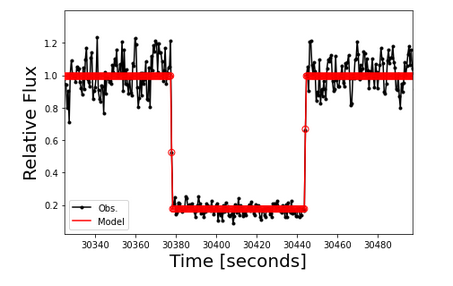
\includegraphics[width=\textwidth]{pngs/Bardecker12.png}
        \centerline{\small (a)}
    \end{minipage}
    \hfill
    \begin{minipage}[b]{0.38\textwidth}
        \centering
        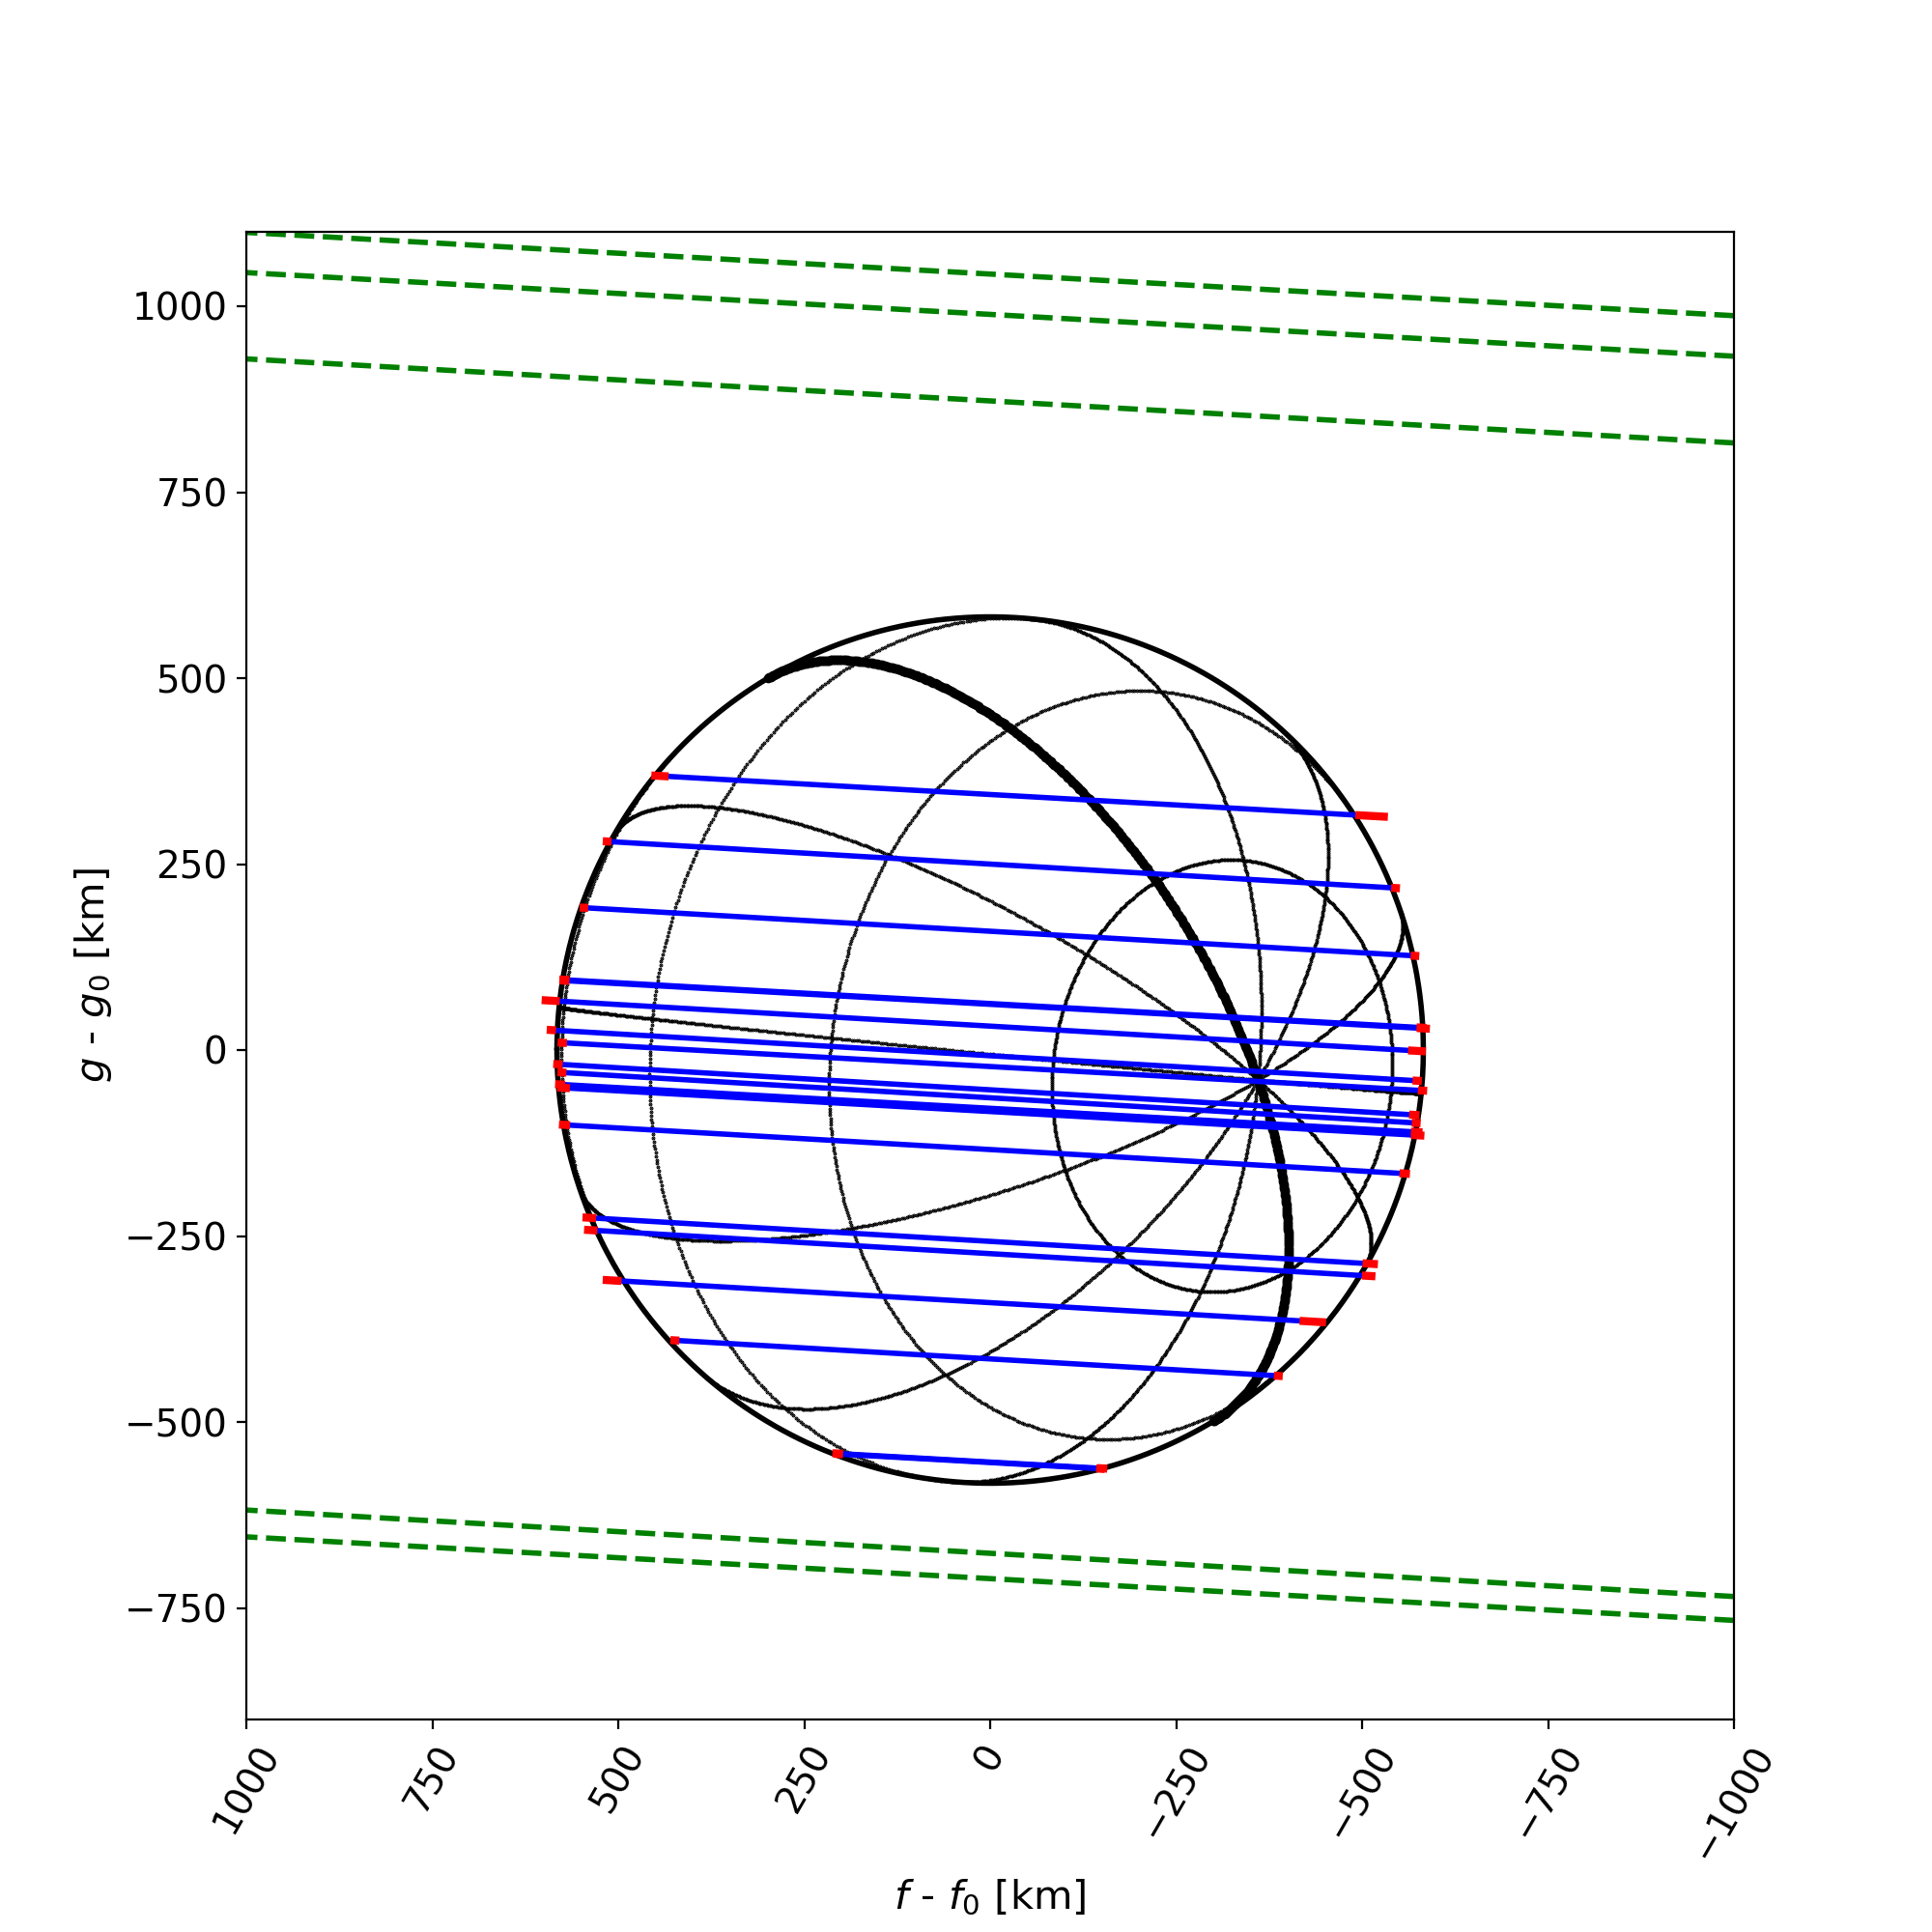
\includegraphics[scale=0.28]{Tese/pngs/LimbFitCircle.png}
        \centerline{\small (b)}
    \end{minipage}
    \caption{(a)~Curva de luz observada (preto) e modelo ajustado (vermelho) para uma das cordas da ocultação por Umbriel em 2020; os instantes de imersão e emersão, marcados por circunferências, definem a geometria da corda \citep{Umbriel2020}. (b)~Perfil do limbo de Umbriel; cada linha azul (incerteza vermelho) corresponde a uma corda projetada no plano do céu \citep{Umbriel2020}.}
    \label{fig:curvas_cordas}
\end{figure}




\textbf{Exemplo numérico: escala de Fresnel.} Para um objeto transnetuniano (TNO) a uma distância típica de $D = 40$\,UA $\approx 6{,}0 \times 10^{12}$\,m, observado no visível ($\lambda = 500$\,nm), a escala de Fresnel é
\[
f = \sqrt{\frac{D\lambda}{2}} \approx \sqrt{\frac{6{,}0 \times 10^{12} \times 5{,}0 \times 10^{-7}}{2}} \approx 1{,}2\;\text{km}.
\]
Essa escala define a resolução espacial efetiva na direção perpendicular à corda: detalhes menores que $f$ são suavizados pela difração. Ainda assim, trata-se de uma resolução da ordem de quilômetros a dezenas de unidades astronômicas de distância - superior à de qualquer telescópio óptico terrestre operando por imageamento direto. É essa capacidade de resolução que torna as ocultações estelares uma ferramenta única para a caracterização de pequenos corpos do Sistema Solar.

\begin{figure}[htbp]
    \centering
    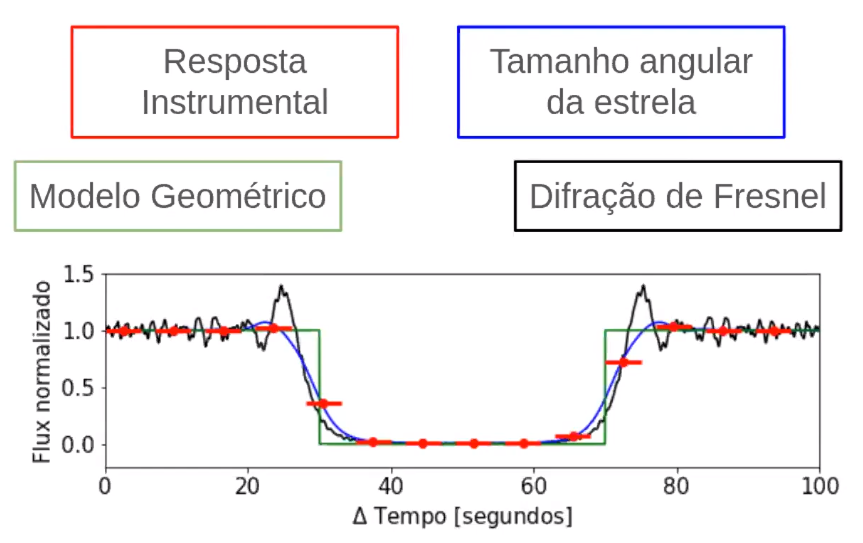
\includegraphics[width=0.55\linewidth]{pngs/ModelosSORA.png}
    \caption{Componentes do modelo de curva de luz utilizado pelo SORA \citep{SORA2022}: difração de Fresnel (azul), tamanho angular da estrela, ciclo de integração do detector e, resultante da combinação dessas componentes, o modelo geométrico (verde). O ajuste simultâneo aos dados observados (pontos vermelhos) permite determinar com precisão os instantes de imersão e emersão, necessários para a reconstrução da forma do corpo.}
    \label{fig:modelo_sora}
\end{figure}

% ---------------------------
\section{Considerações finais do capítulo}
\label{sec:consideracoes_cap2}

Este capítulo situou as ocultações estelares como fenômeno astronômico e as curvas de luz como produto observacional central. Foi destacado o papel da geometria da sombra, das cordas e da precisão astrométrica (Gaia, efemérides) na previsão e no aproveitamento dos eventos; a coleta e o armazenamento dos dados foram descritos em linhas gerais, com remissão ao Capítulo~4 para a arquitetura da \textit{pipeline} e do banco de dados; e foram resumidas as características observacionais das curvas (positiva vs.\ negativa, fatores que afetam a forma, S/N). O volume crescente de dados produzidos por redes de telescópios e catálogos como o Gaia torna \st{inviável} \textcolor{red}{penosa} a triagem manual de todas as curvas de luz; essa escala motiva o desenvolvimento de métodos automatizados de detecção baseados em aprendizado de máquina, cujos fundamentos são apresentados no Capítulo~3 e cuja implementação é detalhada no Capítulo~4. \textcolor{red}{(veja se a frase a seguir se aplica). Notadamente, nos interessam também que sejam apontados eventos tênues e que passaram desapercebidos num primeiro tratamento de curvas de luz (cite aqui os aneis de Quaoar). Um alerta confiável nesses casos é suporte para campanhas observacionais e descobertas importantes.}
